% !TeX root = ./document.tex
\chapter{Úvod, základní pojmy}
Výrok - má pravdivostní hodnotu 0 nebo 1. Mějme A, B výroky:

\begin{figure}[ht!]
	\begin{center}
		\begin{tabular}{|C|C|C|C|C|C|C|}
			\hline
			& & A\land B & & & (A\Rightarrow B) \land (A\Leftarrow B) & \\
			A & B & A\&B & A\lor B & A\Rightarrow B & A\Leftrightarrow B & \lnot A \\
			\hline
			0 & 0 & 0 & 0 & 1 & 1 & 1 \\
			0 & 1 & 0 & 1 & 1 & 0 & 1 \\
			1 & 0 & 0 & 1 & 0 & 0 & 0 \\
			1 & 1 & 1 & 1 & 1 & 1 & 0 \\
			\hline
		\end{tabular}
		\caption{Tabulka pravdivostních hodnot}
	\end{center}
\end{figure}

Důkaz implikace $A\Rightarrow B$:
\begin{enumerate}
	\item přímý: ukážeme, že když $A = 1$, pak $B = 1$
	\item nepřímý: plyne z $\lnot B \Rightarrow \lnot A$
	\item sporem: předpokládáme, že $A = 1 \land B = 0$ a odvodíme spor (např.: $1=2$)
\end{enumerate}

\begin{lemmaAlph}[Čtverec lichého čísla]
	(tvrzení) $\forall n\in \mathbb{N} : n^2~\text{liché} \Rightarrow n~\text{liché}$
\end{lemmaAlph}

\begin{proof}[Důkaz 1]
	Fixuj $n\in \mathbb{N}$. Prvočíselný rozklad:
	\begin{gather}
		n = p_1^{\alpha_1} \cdot \ldots \cdot p_k^{\alpha_k} \\
		n^2 = p_1^{2\alpha_1} \cdot \ldots \cdot p_k^{2\alpha_k} \\
		\forall j \in \left\{1,\ldots,k\right\}: 2 \neq P_j
	\end{gather}
	V rozvoji $n^2$ není $2$, tak v rozvoji $n$ také není (liší se pouze mocninou).
\end{proof}
\begin{proof}[Důkaz 2]
	Chci: $\forall n \in \mathbb{N}: n$ sudé $\Rightarrow n^2$ sudé
	\begin{gather}
		n = 2k, k\in\mathbb{N} \\
		n^2 = 4k^2 = 2(2k^2)
	\end{gather}
\end{proof}
\begin{proof}[Důkaz 3]
	Předpokládejme: $n^2$ liché a $n$ sudé. Pak:
	\begin{gather}
		n^2 + n \text{ liché}  \\
		n(n + 1) \text{ liché a sudé zároveň (spor)}
	\end{gather}  
\end{proof}
O čem budou výroky? O definovaných pojmech:
\begin{itemize}
	\item množina: soubor prvků (př.: množina mužů, žen)
	\item $x\in A$ \quad $x$ je prvkem
	\item $x\notin A$ \quad $\lnot (x\in A)$
	\item $A\subset B$ \quad $A$ je podmnožinou $B$: $\forall x \in A: x \in B$
	\item \O \quad prázdná množina
	\item množinové operace:
	\begin{itemize}
		\item $A\cup B = \left\{x; (x\in A)\lor(x\in B)\right\}$
		\item $A\cap B = \left\{x; (x\in A)\land(x\in B)\right\}$
		\item $A - B = \left\{x; (x\in A)\lor(x\notin B)\right\}$
	\end{itemize}
	\item kvantifikátory:
	\begin{itemize}
		\item $\forall x$ \quad pro všechna $x$
		\item $\exists y$ \quad existuje $y$
		\item př.: $V(x,y)$ je vlastnost, že $y$ je matka $x$. $M$ je množina
			mužů, $Z$ je množina žen.
		\begin{itemize}
			\item $\forall x \in M~\exists y \in Z: V(x,y)$
			\item $\exists y \in Z: \forall x \in M: V(x,y)$
		\end{itemize}
	\end{itemize}
\end{itemize}

\section{Reálná čísla}

\begin{theoremAlph}[Reálná čísla]
	Existuje množina $\mathbb{R}$ s operacemi $\oplus$ a $\otimes$ a relací $<$ tak,
	že splňuje vlastnosti \ref{D-A1} až \ref{D-A4}.
\end{theoremAlph}

\begin{definitionAi}[Algebraická struktura]\labelTheo{D-A1}
	\begin{enumerate}[I]
		\item Komutativita: $\forall x, y \in \mathbb{R}: x + y = y + x;~x\cdot y = y\cdot x$
		\item Asociativita: $\forall x, y, z \in \mathbb{R}: x + (y + z) = (x + y) + z;
			~(x\cdot y)\cdot z = x\cdot (y\cdot z)$
		\item Nulový prvek $\oplus: \exists~0 \in \mathbb{R}: \forall x \in \mathbb{R}: 0 + x = x$ \\
			Jednotka $\otimes: \exists~1 \in \mathbb{R}: \forall x \in \mathbb{R}: 1 \cdot x = x$
		\item Inverzní prvek: $\forall x \in \mathbb{R}, \forall z \in \mathbb{R}~\exists ! y:
			x + y = z$ (právě jedno; ozn. $y = z - x$) \\
			$\forall x, z \in \mathbb{R}, x\neq0 ~\exists ! y \in \mathbb{R}:
			x \cdot y = z$ (ozn. $y = z / x$)
		\item Distributivita: $\forall x, y, z \in \mathbb{R}: x (y + z) = xy + xz$
		\item Násobení nulou: $\forall x \in \mathbb{R}: 0\cdot x = 0$ \\
			$\forall x, y \in \mathbb{R}: x\cdot y = 0 \Rightarrow ((x = 0) \lor (y = 0))$
	\end{enumerate}
\end{definitionAi}
Další vlastnosti lze odvodit:
\begin{alignat}{1}
	-(-x) &= x \\
	-(x\cdot y) &= (-x)\cdot y
\end{alignat}
Další značení:
\begin{alignat}{1}
	x^n &= x\cdot x\cdot \text{...} \cdot x \text{~($n$-krát)} \\
	-x &= 0 - x \\
	\forall x \neq 0: x^{-1} &= \frac{1}{x} \\
	\forall x \neq 0: x^{-n} &= \left( \frac{1}{x} \right)^n
\end{alignat}

I. - IV. říká $(\mathbb{R}, +)$ a $(\mathbb{R} - \left\{0\right\}, \cdot)$ jsou grupy.

I. - VI. říká $(\mathbb{R}, +, \cdot)$ je těleso.

Ověřte, že Vlastnost \ref{D-A1} platí pro $\mathbb{C}$ (komplexní čísla).

\begin{example}
	Definujme $\mathbb{C} = \left\{z = (z_1, z_2); z_1, z_2 \in \mathbb{R}\right\}$ a
	operace $\oplus, \otimes$. $\forall z, u \in \mathbb{C}:$
	\begin{alignat}{1}
		(z_1, z_2) + (u_1, u_2) &= (z_1 + u_1, z_2, u_2) \\
		(z_1, z_2) \cdot (u_1, u_2) &= (z_1u_1 - z_2u_2, z_1u_2 + z_2u_1)
	\end{alignat}
	Nulový prvek: $(0, 0)$
	
	Jednotkový prvek: $(1, 0)$

	Lze zapisovat $z\in \mathbb{C}$, $z = (z_1, z_2)$, ozn. $z = z_1 + iz_2$ pro $i^2 = -1$.
\end{example}
\begin{definitionAi}[Uspořádání]\labelTheo{D-A2}
	\begin{enumerate}[I]
		\item Relace: $\forall x, y \in \mathbb{R}$ nastane právě jedna z možností: \\
		$(x<y)$ nebo $(x>y)$ nebo $(x=y)$
		\item Tranzitivita: $(x<y) \land (y<z) \Rightarrow (x<z)$
		\item\label{D-A2-3} Vztah uspořádání a sčítání: $(x<y) \Rightarrow x+z < y+z$
		\item\label{D-A2-4} Vztah relace k násobení: $(0<x) \land (0<y) \Rightarrow 0 < xy$
	\end{enumerate}
\end{definitionAi}

Značení:
\begin{itemize}
	\item $x>y \Leftrightarrow y<x$
	\item $(x\leq y) \Leftrightarrow (x<y) \lor (x=y)$
	\item $(x\geq y) \Leftrightarrow (x>y) \lor (x=y)$
\end{itemize}

Lze odvodit další pravidla:
\begin{equation}\label{RelationsOfNegatives}
	x<y \Leftrightarrow -x > -y
\end{equation}
\begin{proof}
	\begin{alignat*}{2}
		x&<y \\
		x-x&<y-x &&\text{\quad /bod \ref{D-A2-3}} \\
		0&<y-x \\
		0-y&<y-y-x &&\text{\quad /bod \ref{D-A2-3}} \\
		-y&<-x \\
		-x&>-y &&\text{\quad funguje $\Leftrightarrow$} \\
	\end{alignat*}
\end{proof}

DÚ:
\begin{equation}
	\forall x \in \mathbb{R}: x>0 \Rightarrow \frac{1}{x}>0
\end{equation}
\begin{proof}
	Sporem:
	\begin{alignat*}{1}
		x>0 &\text{ a } \frac{1}{x}<0 \\
		-\frac{1}{x}&>0 \\
		0&<x\cdot\left(-\frac{1}{x}\right) = -1 \\
		1 &< 0
	\end{alignat*}
	Pokud $0<1$, pak spor! $0<1<0$.

	Máme $0<-1 \xRightarrow{\ref{D-A2-4}} 0<(-1)(-1) = 1$
\end{proof}

\begin{example}
	Komplexní čísla nelze uspořádat podle Vlastnosti \ref{D-A2}
\end{example}
\begin{proof}
	Sporem: Předpokládejme, že to lze.
	\begin{alignat*}{1}
		i&<0 \\
		(0,1)&<(0,0) \\
		-i>0 &\xRightarrow{\ref*{D-A2}-\ref{D-A2-4}} 0<(-i)(-i) = -1
	\end{alignat*}
	Pozn.: $i>0 \xRightarrow{\ref*{D-A2}-\ref{D-A2-4}} 0<(i)(i) = -1$
\end{proof}

\section{Význačné podmnožiny \texorpdfstring{$\mathbb{R}$}{R}}
\begin{itemize}
	\item $\mathbb{N} = \left\{1,2,\dots\right\}$\quad přirozená čísla
	\item $\mathbb{Z} = \left\{0,-1,-2,\dots\right\}\cup\mathbb{N}$\quad celá čísla
	\item $\mathbb{Q} = \left\{\frac{p}{q}: p\in\mathbb{Z}, q\in\mathbb{N}\right\}$\quad racionální čísla
	\item $\mathbb{R} - \mathbb{Q}$\quad iracionální čísla
\end{itemize}

Poznámka: $\mathbb{Q}$ má obě vlastnosti \ref{D-A1}, \ref{D-A2}

Intervaly:
\begin{itemize}
	\item $(a,b) = \left\{x\in\mathbb{R}; a<x<b\right\}$\quad otevřený
	\item $[a,b] = (a,b)\cup\left\{a,b\right\}$\quad uzavřený
	\item $[a,b), (a,b]$\quad polootevřené
	\item $(a,+\infty) = \left\{x\in\mathbb{R}; x>a\right\}$\quad neomezený otevřený
	\item $(-\infty, a) = \left\{x\in\mathbb{R}; x<a\right\}$\quad neomezený otevřený
	\item podobně: $[a, +\infty), (-\infty, a]$\quad neomezený uzavřený
\end{itemize}

\begin{definition}[Absolutní hodnota]
	Pro $x\in\mathbb{R}$ definuji
	\[  % Means \begin{equation*} and \end{equation*} with amsmath loaded.
	\abs{x} =
	\begin{cases}
		x &\quad\text{ pokud } x\geq 0 \\
		-x &\quad\text{ pokud } x<0
	\end{cases}
	\]
\end{definition}

\begin{lemma}[Vlastnosti absolutní hodnoty]\labelTheo{L-abs}
	Nechť $a>0$, pak $\abs{x}<a$ právě \\ když $-a<x<a$
\end{lemma}
\begin{proof}
	\begin{enumerate}
		\item\label{L-abs-P1} Ať $x\geq 0$ pak $\abs{x}=x$ a máme ukázat, že $x<a \Leftrightarrow -a<x<a$ \\
			"$\Leftarrow$" jasná | "$\Rightarrow$" víme $-a<0\leq x<a$
		\item Ať $x<0$, pak $\abs{x} = -x$ a máme ukázat, že $-x<a \Leftrightarrow -a<x<a$ \\
			$x>-a$ pak pokračujeme podobně jako \ref{L-abs-P1}.: $-a<x<0<a$
	\end{enumerate}
\end{proof}

\begin{theorem}[Trojúhelníková nerovnost]\labelTheo{T-triangleInequality}
	\begin{alignat}{1}
		\abs{x+y} &\leq  \abs{x} + \abs{y} \label{T-triangleInequality-1} \\
		\abs{x-y} &\leq  \abs{x} + \abs{y} \label{T-triangleInequality-2} \\
		\abs{x+y} &\geq  \abs{\abs{x} - \abs{y}} \label{T-triangleInequality-3} \\
		\abs{x-y} &\geq  \abs{\abs{x} - \abs{y}} \label{T-triangleInequality-4}
	\end{alignat}
\end{theorem}
\begin{proof}
	\ref{T-triangleInequality-1} a \ref{T-triangleInequality-2} plyne z Lemma \ref{L-abs}
	
	\ref{T-triangleInequality-3} a \ref{T-triangleInequality-4} plyne z předešlého řádku pomocí triku
	\begin{alignat}{1}
		x &= x+y-y \\
		\abs{x} &=\abs{x+y-y}\leq\abs{x+y}+\abs{y} \\
		\abs{y} &\leq\abs{x+y}+\abs{x} \\
		\abs{x}-\abs{y} &\leq\abs{x+y} \\
		\abs{y}-\abs{x} &\leq\abs{x+y}~/\cdot(-1) \label{T-triangleInequality-P126} \\
		\abs{x}-\abs{y} &\geq-\abs{x+y}~
			\text{plyne z \ref{T-triangleInequality-P126} a \ref{RelationsOfNegatives}}
	\end{alignat}
\end{proof}

\begin{definition}[Maximum]
	Nechť $M\subset\mathbb{R}$
	\begin{itemize}
		\item $x\in M$ nazveme maximum $M$, pokud $\forall y\in M: y\leq x$ \\
			Ozn. $x=max~M$ \\
			Př.: $(0,1)$ nemá max
		\item $K\in\mathbb{R}$ nazveme horní odhad $M$, pokud $\forall x\in M: x\leq K$ \\
			Př.: $(0,1)$ má horní odhad 4, 1, \dots
	\end{itemize}
\end{definition}

\begin{lemma}[Jednoznačnost max]
	Existuje nejvýše 1 max. $M\subset\mathbb{R}$
\end{lemma}
\begin{proof}
	Ať existují dvě: $x_1, x_2\in M$ maxima
	\begin{alignat}{1}
		x_1 \text{je max; }x_2\in M &\Rightarrow x_1\geq x_2 \\
		x_2 \text{je max; }x_1\in M &\Rightarrow x_2\geq x_1 \\
		\Rightarrow x_1\leq x_2\leq x_1
	\end{alignat}
	Tedy $x_1=x_2$
\end{proof}

Pozn.: analogicky def. minimum a dolní odhad.

\begin{definition}[Supremum]
	Číslo $s\in\mathbb{R}$ nazvu supremem množiny $M\subset\mathbb{R}$, pokud
	\begin{enumerate}[I]
		\item\label{D-supremum-1} $\forall x\in M: x\leq s$
		\item\label{D-supremum-2} $\forall s'<s, s'\in\mathbb{R}: \exists x\in M: s'<x$
	\end{enumerate}
	Supremum $M$ značíme $s=sup~M$
\end{definition}

Pozn.: \ref{D-supremum-1} říká, že $s$ je horní odhad, \ref{D-supremum-2} říká,
že $s$ je nejmenší možný horní odhad

Pozn.: pokud supremum náleží do intervalu, je to jeho maximum

\begin{definition}[Infimum]
	Nechť $M\subset\mathbb{R}$. řekneme, že $s\in\mathbb{R}$ je infimum množiny $M$
	(ozn. $inf~M$), pokud
	\begin{enumerate}[I]
		\item\label{D-infimum-1} $\forall x\in M: s\leq x$
		\item\label{D-infimum-2} $\forall s'>s, s'\in\mathbb{R}: \exists x<s': x\in M$
	\end{enumerate}
	Infimum $M$ značíme $s=inf~M$
\end{definition}

\begin{definitionAi}[Supremum a infimum]\labelTheo{D-A3}
	Každá neprázdná shora omezená $M\subset\mathbb{R}$ má supremum v $\mathbb{R}$.
	Každá neprázdná zdola omezená $M\subset\mathbb{R}$ má infimum v $\mathbb{R}$.
\end{definitionAi}

\begin{definition}[Odmocnina]\labelTheo{D-sqrt}
	\begin{enumerate}
		\item Nechť $a>0$ a $n$ sudé, $n\in\mathbb{N}$, pak existuje právě jedno číslo $b>0: b^n=a$
		\item Nechť $a>0$ a $n$ liché, $n\in\mathbb{N}$, pak existuje právě jedno číslo $b\in\mathbb{R}: b^n=a$
	\end{enumerate}
	Značení: $b=\sqrt[n]{a}$
\end{definition}

\begin{lemmaAlph}[Čtverec dělitelný třema]\labelTheo{L-divisibilityByThree}
	% \[$k^2$ je dělitelné $3 \Rightarrow k$ je děl. $3$\]
	$k^2 \text{ je dělitelné }3\Rightarrow k \text{ je děl. }3$
\end{lemmaAlph}
\begin{proof}
	Jak zapsat $k$? $\exists m\in\mathbb{Z}:$
	\begin{alignat}{2}
		k &= 3m+0 &&k^2\text{ je děl. $3$}\\
		k &= 3m+1 \Rightarrow k^2=9m^2+6m+1 \quad&&\text{není děl. $3$} \\
		k &= 3m+2 \Rightarrow k^2=9m^2+12m+4 \quad&&\text{není děl. $3$}
	\end{alignat}
\end{proof}

\begin{theorem}[Iracionální čísla]
	Existují iracionální čísla
\end{theorem}
\begin{proof}
	Tvrdíme, že $\sqrt{3}$ není racionální. Sporem:
	\begin{alignat}{1}
		\text{Ať $\sqrt{3}$ je rac.} &\Rightarrow\exists k\in\mathbb{Z}, l\in\mathbb{N}
		\text{ nesoudělná: }\sqrt{3}=\frac{k}{l} \\
		3=\frac{k^2}{l^2} &\Rightarrow k^2=3l^2 \\
		k^2 \text{ je dělitelné }3 &\xRightarrow{L\ref{L-divisibilityByThree}} k\text{ je děl. }3 \\
		n\in\mathbb{Z}: \left(k=3n\Rightarrow k^2=9n^2\right) &\Rightarrow k^2 \text{ je děl }9 \\
		k^2=9n^2=3l^2 &\Rightarrow l^2=3n^2 \\
		l^2 \text{ je děl. }3 &\xRightarrow{L\ref{L-divisibilityByThree}} l\text{ je děl. }3
	\end{alignat}
	Což je spor, protože $k$, $l$ jsou nesoudělná.
\end{proof}

\begin{definitionAi}[Vlastnosti \texorpdfstring{$\mathbb{N}$}{N}]\labelTheo{D-A4}
	\begin{enumerate}[I]
		\item\label{D-A4-1} $\forall x\in\mathbb{R}\exists n\in\mathbb{N}: x<n$
		\item Princip indukce: nechť $M\subset\mathbb{N}$ a
			\begin{enumerate}
				\item $1\in M$
				\item $n\in M \Rightarrow n+1\in M$
			\end{enumerate}
			Pak $m=\mathbb{N}$
	\end{enumerate}
\end{definitionAi}

Pozn.:Vlastnost \ref{D-A4-1} plyne z vlastnosti \ref{D-A3}

Pozn.: Archimédova vlastnost:
\begin{equation}
	\forall m\in\mathbb{N}, \forall \epsilon>0 \text{ (tedy reálné) }\exists n\in\mathbb{N}:n\epsilon>m
\end{equation}
\begin{proof}
	Polož $x=m/\epsilon$ v \ref{D-A4-1}
\end{proof}

\begin{theorem}[Velikost intervalu]
Každý otevřený interval obsahuje nekonečně \\ racionálních i nekonečně iracionálních čísel.
\end{theorem}
\begin{proof}
	Ve zkratce:
	\begin{alignat}{2}
		\frac{k}{l}&+\frac{n}{n+1}\frac{1}{l} &&\quad\text{ je racionální }\forall n\in\mathbb{N} \\
		\frac{k}{l}&+\frac{\sqrt{3}}{3}\frac{n}{n+1}\frac{1}{l} &&\quad\text{ je iracionální }\forall n\in\mathbb{N}
	\end{alignat}
	\begin{figure}[ht!]
		\begin{center}
			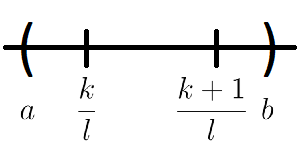
\includegraphics[width=0.4\textwidth,keepaspectratio]{../img/chapter1/interval.png}
			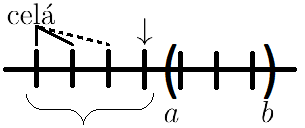
\includegraphics[width=0.4\textwidth,keepaspectratio]{../img/chapter1/interval2.png}
			% \caption{}
		\end{center}
	\end{figure}\FloatBarrier
	
	Mějme otevřený interval $(a,b)$. Stačí mít rac. č. $k/l$ tak, aby \\$k/l,~(k+1)/l\in(a,b)$.
	\begin{alignat*}{2}
		\text{Jak hledám $l$? }&\quad\frac{1}{l}<\frac{b-a}{2}
			&&\quad\text{plyne z \ref*{D-A4}-\ref{D-A4-1} pomocí }l>\frac{2}{b-a}\\
		\text{Jak hledám $k$? }&\quad\text{def. }M=\left\{n\in\mathbb{Z};\frac{n}{l}<a\right\}
			&&\quad\text{podle \ref{D-A3} }\exists s\in\mathbb{R}:s=sup~M
	\end{alignat*}
	Tvrdíme: $s\in M$:

	Podle \hyperref[D-supremum-2]{druhé vlastnosti suprema}: $\forall s'<s~\exists n\in M:s'<n$ \\
	Volím $s'\in\left(s-\frac{1}{2},s\right)$, pak $\exists n'\in M: s'<n'$. Zafixuji $n'$ a tvrdím:
	\begin{equation}\label{T-intervalSize-P-144}
		\forall s'\in (s-\frac{1}{2},s): s'<n'\leq s
	\end{equation}
	A tedy $s\leq n'\leq s$. Definujme
	\begin{alignat}{1}
		k&:=s+1 \Rightarrow \frac{k}{l}\in (a,b) \\
		k+1&:=s+2 \Rightarrow \frac{k+1}{l}\in (a,b) \\
		&\text{Potom:} \nonumber\\
		a<\frac{k}{l}<\frac{k+s}{l}&=\frac{s+2}{l}<a+\frac{2}{l}<a+b-1=b  % ???
	\end{alignat}
\end{proof}

\begin{proof}
	\ref{T-intervalSize-P-144} Vol. $s''\in (s-\frac{1}{2},s)$ pak $\exists n''\in M: s''<n''$
	\begin{alignat}{3}
		s-\frac{1}{2}&<s'&<n'&\leq s \\
		s-\frac{1}{2}&<s''&<n''&\leq s
	\end{alignat}
	Tedy:
	\begin{alignat}{1}
		n',n'' \in (s-\frac{1}{2},s]\cap\mathbb{Z}\Rightarrow n'=n''
	\end{alignat}
\end{proof}
